\chapter{Methodology}

This chapter explains the complete pipeline of the NLGCN 
framework for influential node detection in un-weighted graphs 
\cite{guo2026}. This pipeline converts a raw graph into a structured 
tensor representation, which is then processed by an 
attention-augmented convolutional neural network to produce node 
influence scores \cite{guo2026, tu2025}.

The framework of NLGCN consists of three main stages: 
(a) node feature extraction, (b) structural channel set construction 
embedded with feature information, and (c) model prediction via 
attention and convolutional layers \cite{guo2026}. Figure~\ref{fig:nlgcn_arch} 
illustrates this complete pipeline.

\begin{figure}[h]
    \centering
    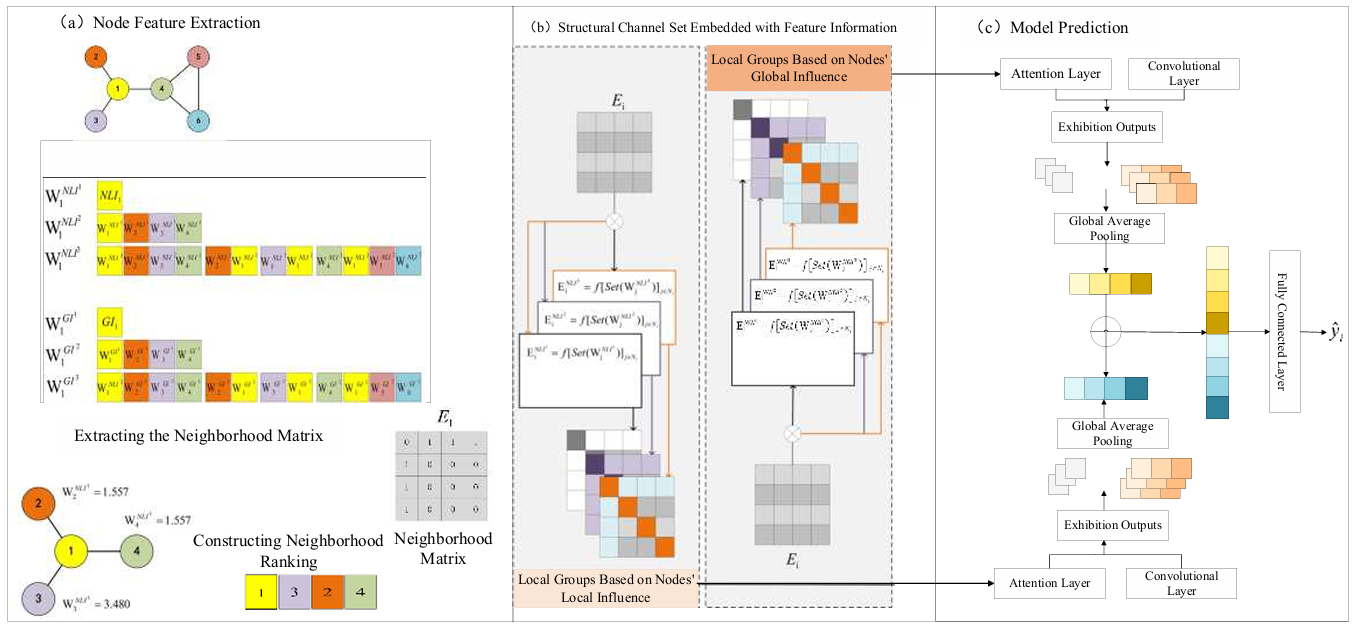
\includegraphics[width=\textwidth]{architecture.png}
    \caption{Basic Framework of the NLGCN model showing (a) Node 
    Feature Extraction, (b) Structural Channel Set Embedded with 
    Feature Information, and (c) Model Prediction \cite{guo2026}.}
    \label{fig:nlgcn_arch}
\end{figure}

\section{Graph Representation}

The input network is represented as an undirected graph $G = (V, E)$, 
where $V$ denotes the set of nodes and $E$ denotes the set of edges 
connecting nodes \cite{hafiene2020, patel2025}. The structural 
information of the graph is captured using an adjacency matrix $A$, 
where:

\begin{equation}
A_{ij} =
\begin{cases}
1 & \text{if there exists an edge between node } i \text{ and node } j \\
0 & \text{otherwise}
\end{cases}
\end{equation}

This representation allows efficient computation of node connectivity, 
degree, and neighbourhood relationships \cite{chen2012, farooq2018}.

\section{Local Node Influence (NLI)}

Local Node Influence (NLI) measures the importance of a node based on 
its immediate neighbourhood structure \cite{guo2026}. It captures how 
strongly a node is connected to its nearby nodes. The NLI for a node 
$i$ is defined as:

\begin{equation}
\text{NLI}_i = \frac{d(v_i) \cdot \log\!\left(\displaystyle\sum_{j 
\in N(i)} \exp\!\left(N_i(v_j)\right)\right)}{n}
\end{equation}

\noindent where:
\begin{itemize}
    \item $d(v_i)$ is the degree of node $i$,
    \item $N(i)$ represents the set of neighbours of node $i$,
    \item $n$ is the total number of nodes in the graph.
\end{itemize}

The exponential term amplifies the contribution of highly influential 
neighbours, while the logarithmic scaling prevents extremely large 
values \cite{guo2026}. Multiplying by the node degree ensures that 
nodes with more connections exert higher influence \cite{ chen2012}. Thus, NLI captures local connectivity strength and the 
influence contribution of immediate neighbours.

\section{Node Global Influence (NGI)}

Node Global Influence (NGI) captures the influence of a node across 
the entire network by incorporating both node degree and shortest path 
distances \cite{guo2026, mukhtar}. The NGI is defined as:

\begin{equation}
\text{NGI}_i = \sum_{i \neq j} \frac {\sqrt{d(v_j) + \alpha}}{{d_{ij}}}
\end{equation}

\noindent where:
\begin{itemize}
    \item $d(v_j)$ is the degree of node $j$,
    \item $d_{ij}$ is the shortest path distance between nodes $i$ 
    and $j$,
    \item $\alpha$ is a balancing constant.
\end{itemize}

Nodes with higher degree contribute more influence; however, their 
contribution decreases with distance, ensuring that closer nodes have 
a stronger impact \cite{guo2026, chen2012}. The square root in the 
denominator reduces the rate of decay, allowing distant nodes to still 
contribute meaningfully. Thus, NGI captures global connectivity and 
network-wide influence propagation \cite{mukhtar}.

\section{Multi-Scale Feature Construction}

To capture hierarchical structural information, multi-scale features 
are constructed using iterative neighbourhood aggregation \cite{guo2026, 
tu2025}. This approach is inspired by the idea that a node's influence 
extends beyond its immediate neighbours to higher-order structural 
contexts \cite{zhang2019gcn}.

\noindent \textbf{NLI-based multi-scale features:}
\begin{align}
W_{\text{NLI}1}(i) &= \text{NLI}_i \\
W_{\text{NLI}2}(i) &= W_{\text{NLI}1}(i) + \sum_{j \in N(i)} 
W_{\text{NLI}1}(j) \\
W_{\text{NLI}3}(i) &= W_{\text{NLI}2}(i) + \sum_{j \in N(i)} 
W_{\text{NLI}2}(j)
\end{align}

\noindent \textbf{NGI-based multi-scale features} are constructed 
analogously \cite{guo2026}:
\begin{align}
W_{\text{NGI}1} &= \text{NGI} \\
W_{\text{NGI}2} &= \text{aggregation over neighbours} \\
W_{\text{NGI}3} &= \text{higher-order aggregation}
\end{align}

Although only immediate neighbours are explicitly used in each step, 
repeated aggregation propagates information across multiple hops 
\cite{zhang2019gcn}. This enables the model to capture both 
local and global structural patterns indirectly \cite{guo2026}.

\section{Neighbourhood Matrix Construction}

For each node $i$, a neighbourhood subgraph is constructed using its 
top-$L$ most important neighbours, ranked by their feature values 
\cite{guo2026, tu2025}. The neighbourhood matrix is defined as:

\begin{equation}
A_{ij} =
\begin{cases}
1 & \text{if there exists an edge between node } i \text{ and node } j \\
0 & \text{otherwise}
\end{cases}
\end{equation}

The resulting matrix has size $(L+1) \times (L+1)$, where one 
row/column corresponds to the target node and the remaining correspond 
to the selected neighbours \cite{guo2026}. This step transforms 
irregular graph structures into fixed-size matrices, making them 
suitable for processing by convolutional neural networks \cite{tu2025, 
patel2025}.

\section{Structural Channel Construction}

Six structural channels are constructed by embedding feature values 
into the neighbourhood matrix \cite{guo2026}:
\begin{itemize}
    \item $\text{NLI}_1$, $\text{NLI}_2$, $\text{NLI}_3$
    \item $\text{NGI}_1$, $\text{NGI}_2$, $\text{NGI}_3$
\end{itemize}

The embedding rule is as follows \cite{guo2026}:
\begin{itemize}
    \item Diagonal elements carry the feature value of the target 
    node $i$.
    \item Off-diagonal elements carry the feature value of a neighbour 
    if an edge exists.
    \item Otherwise, the element is set to $0$.
\end{itemize}

This creates a structured spatial representation where both node 
features and connectivity are encoded, analogous to image channels 
in computer vision \cite{tu2025}.

\section{Channel Tensor Formation}

All six structural channels are stacked to form a 3-dimensional 
input tensor \cite{guo2026}:

\begin{equation}
\text{Input Tensor Size} = 6 \times (L+1) \times (L+1)
\end{equation}

Each channel represents a distinct structural perspective. Stacking 
them allows the model to jointly learn from multiple feature types 
simultaneously \cite{tu2025, zhang2019gcn}.

\section{Channel Attention Mechanism}

To dynamically select the most informative channels, a channel 
attention mechanism is applied to the input tensor \cite{
guo2026}. This mechanism is inspired by the Squeeze-and-Excitation 
Networks, adapted here for structural graph 
channels. The procedure is as follows:

\begin{enumerate}
    \item \textbf{Global Average Pooling:} Compute the mean value 
    $z_c$ for each channel $c$ .
    \item \textbf{Fully Connected Transformation:}
    \begin{equation}
        \mathbf{y} = \sigma\!\left(W_2 \cdot 
        \text{ReLU}(W_1 \cdot \mathbf{z})\right)
    \end{equation}
    where $W_1$ and $W_2$ are learnable weight matrices and $\sigma$ 
    denotes the sigmoid activation \cite{ guo2026}.
    \item \textbf{Channel-wise Scaling:}
    \begin{equation}
        \text{output} = \text{input} \times \mathbf{y}
    \end{equation}
\end{enumerate}

The model learns scalar weights for each channel. Important channels 
receive higher attention weights, while less relevant ones are 
suppressed , allowing the network to focus on the 
most discriminative structural perspectives \cite{guo2026}.

\section{NLGCN Model Architecture}

The Neural Local Graph Convolutional Network (NLGCN) processes the 
attention-weighted channel tensor through the following pipeline 
\cite{guo2026}. As illustrated in Figure~\ref{fig:nlgcn_pipeline}, 
the input tensor passes sequentially through an attention mechanism, 
convolutional layers, pooling layers, and fully connected layers to 
produce the final influence score.

\begin{figure}[h]
    \centering
    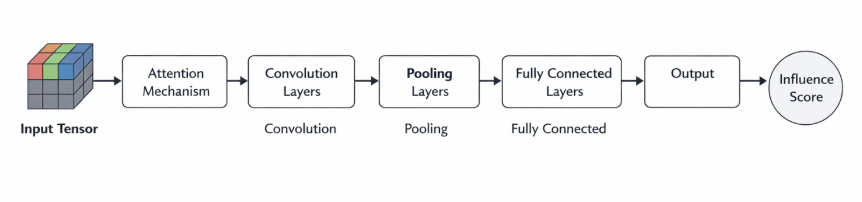
\includegraphics[width=\textwidth]{pipeline.png}
    \caption{NLGCN model processing pipeline}
    \label{fig:nlgcn_pipeline}
\end{figure}

\begin{itemize}
    \item \textbf{Convolution layers} extract local structural patterns 
    from the tensor \cite{tu2025, zhang2019gcn}.
    \item \textbf{Pooling layers} reduce spatial dimensionality and 
    improve generalization \cite{tu2025}.
    \item \textbf{Fully connected layers} map the learned features to 
    a single scalar influence score \cite{guo2026, patel2025}.
\end{itemize}

The final output is a real-valued scalar representing the predicted 
influence score of a node \cite{guo2026}.

\section{SIR-Based Label Generation}

Ground truth influence labels are generated using the 
Susceptible-Infected-Recovered (SIR) epidemic diffusion model 
\cite{ chen2012}. The epidemic threshold is computed as 
\cite{guo2026}:

\begin{equation}
\beta_c = \frac{\langle k \rangle}{\langle k^2 \rangle - 
\langle k \rangle}
\end{equation}

\noindent where $\langle k \rangle$ is the average node degree and 
$\langle k^2 \rangle$ is the average squared degree. Simulation 
parameters are set as $\beta = 1.5\,\beta_c$ and $\mu = 1$ 
\cite{guo2026, patel2025}.

The simulation procedure is \cite{ chen2012}:
\begin{enumerate}
    \item Each node is selected in turn as the initially infected node.
    \item Infection spreads to susceptible neighbours probabilistically 
    with rate $\beta$.
    \item The process is repeated for a fixed number of runs 
    (e.g., 500).
    \item The average number of recovered nodes across runs is taken 
    as the influence score of the initial node.
\end{enumerate}

Nodes that infect a greater number of nodes on average are considered 
more influential \cite{chen2012}.

\section{Model Training}

The NLGCN model is trained using supervised regression \cite{guo2026}. 
The loss function is the Mean Squared Error (MSE):

\begin{equation}
\mathcal{L} = \frac{1}{n} \sum_{i=1}^{n} \left(\hat{y}_i - 
y_i\right)^2
\end{equation}

\noindent where $\hat{y}_i$ is the predicted influence score and $y_i$ 
is the SIR-derived ground truth label \cite{guo2026}. The Adam 
optimizer is used to update model parameters via backpropagation 
\cite{tu2025, patel2025}.

\section{Evaluation Metrics}

\subsection{Kendall Tau Correlation}

The Kendall Tau ($\tau$) coefficient measures the ranking similarity 
between the predicted influence scores and the true SIR-based 
influence scores \cite{ mukhtar}:

\begin{equation}
\tau = \frac{C - D}{\frac{1}{2}\,n(n-1)}
\end{equation}

\noindent where $C$ is the number of concordant pairs and $D$ is the 
number of discordant pairs . A value of $\tau$ close to 
$1$ indicates near-perfect ranking agreement \cite{guo2026, mukhtar}.

\subsection{Top-$N$ Spread Evaluation}

The practical effectiveness of the model is evaluated using the 
Top-$N$ spread metric \cite{guo2026, chen2012}:
\begin{enumerate}
    \item Selecting top-$N$ nodes ranked based on the predicted influence score.
    \item Running SIR simulations with these nodes as initial spreaders.
    \item Measuring the total number of infected nodes (spread) averaged 
    over multiple runs \cite{chen2012}.
\end{enumerate}

This metric directly evaluates the real world utility of the predicted 
rankings \cite{guo2026}.